\section{Methodology}
	
	\subsection{Hardware ${}^{\ref{HardwareSource}}$ }

	\begin{enumerate}[topsep=-2pt, itemsep=10mm]
		\item \textbf{Raspberry Pi 3 Model B:} 
		
			The Raspberry Pi 3 is a hobbyist microcontroller board which can be used for a variety of embedded systems projects. 
		
			It's specifications ${}^{\cite{RPi3BSpecs}}$ include:
			\begin{description}[font=\quad $\circ$, topsep=-2pt, itemsep=2pt]
				\item Broadcom BCM2837 64bit ARMv7 Quad Core Processor powered Single Board computer running at 1.2GHz
				\item 1 GB RAM
				\item BCM43143 WiFi on board
				\item 4 USB 2.0 ports
				\item 40 GPIO pins${}^{\ref{fig: Raspberry Pi 3B pin diagram}}$ (General Purpose Input Output)
				\item Full HDMI port
				\item Micro SD card slot (an 8Gb SanDisk MicroSD was used)
			\end{description}
			
			\begin{figure}[!h]
				\centering
				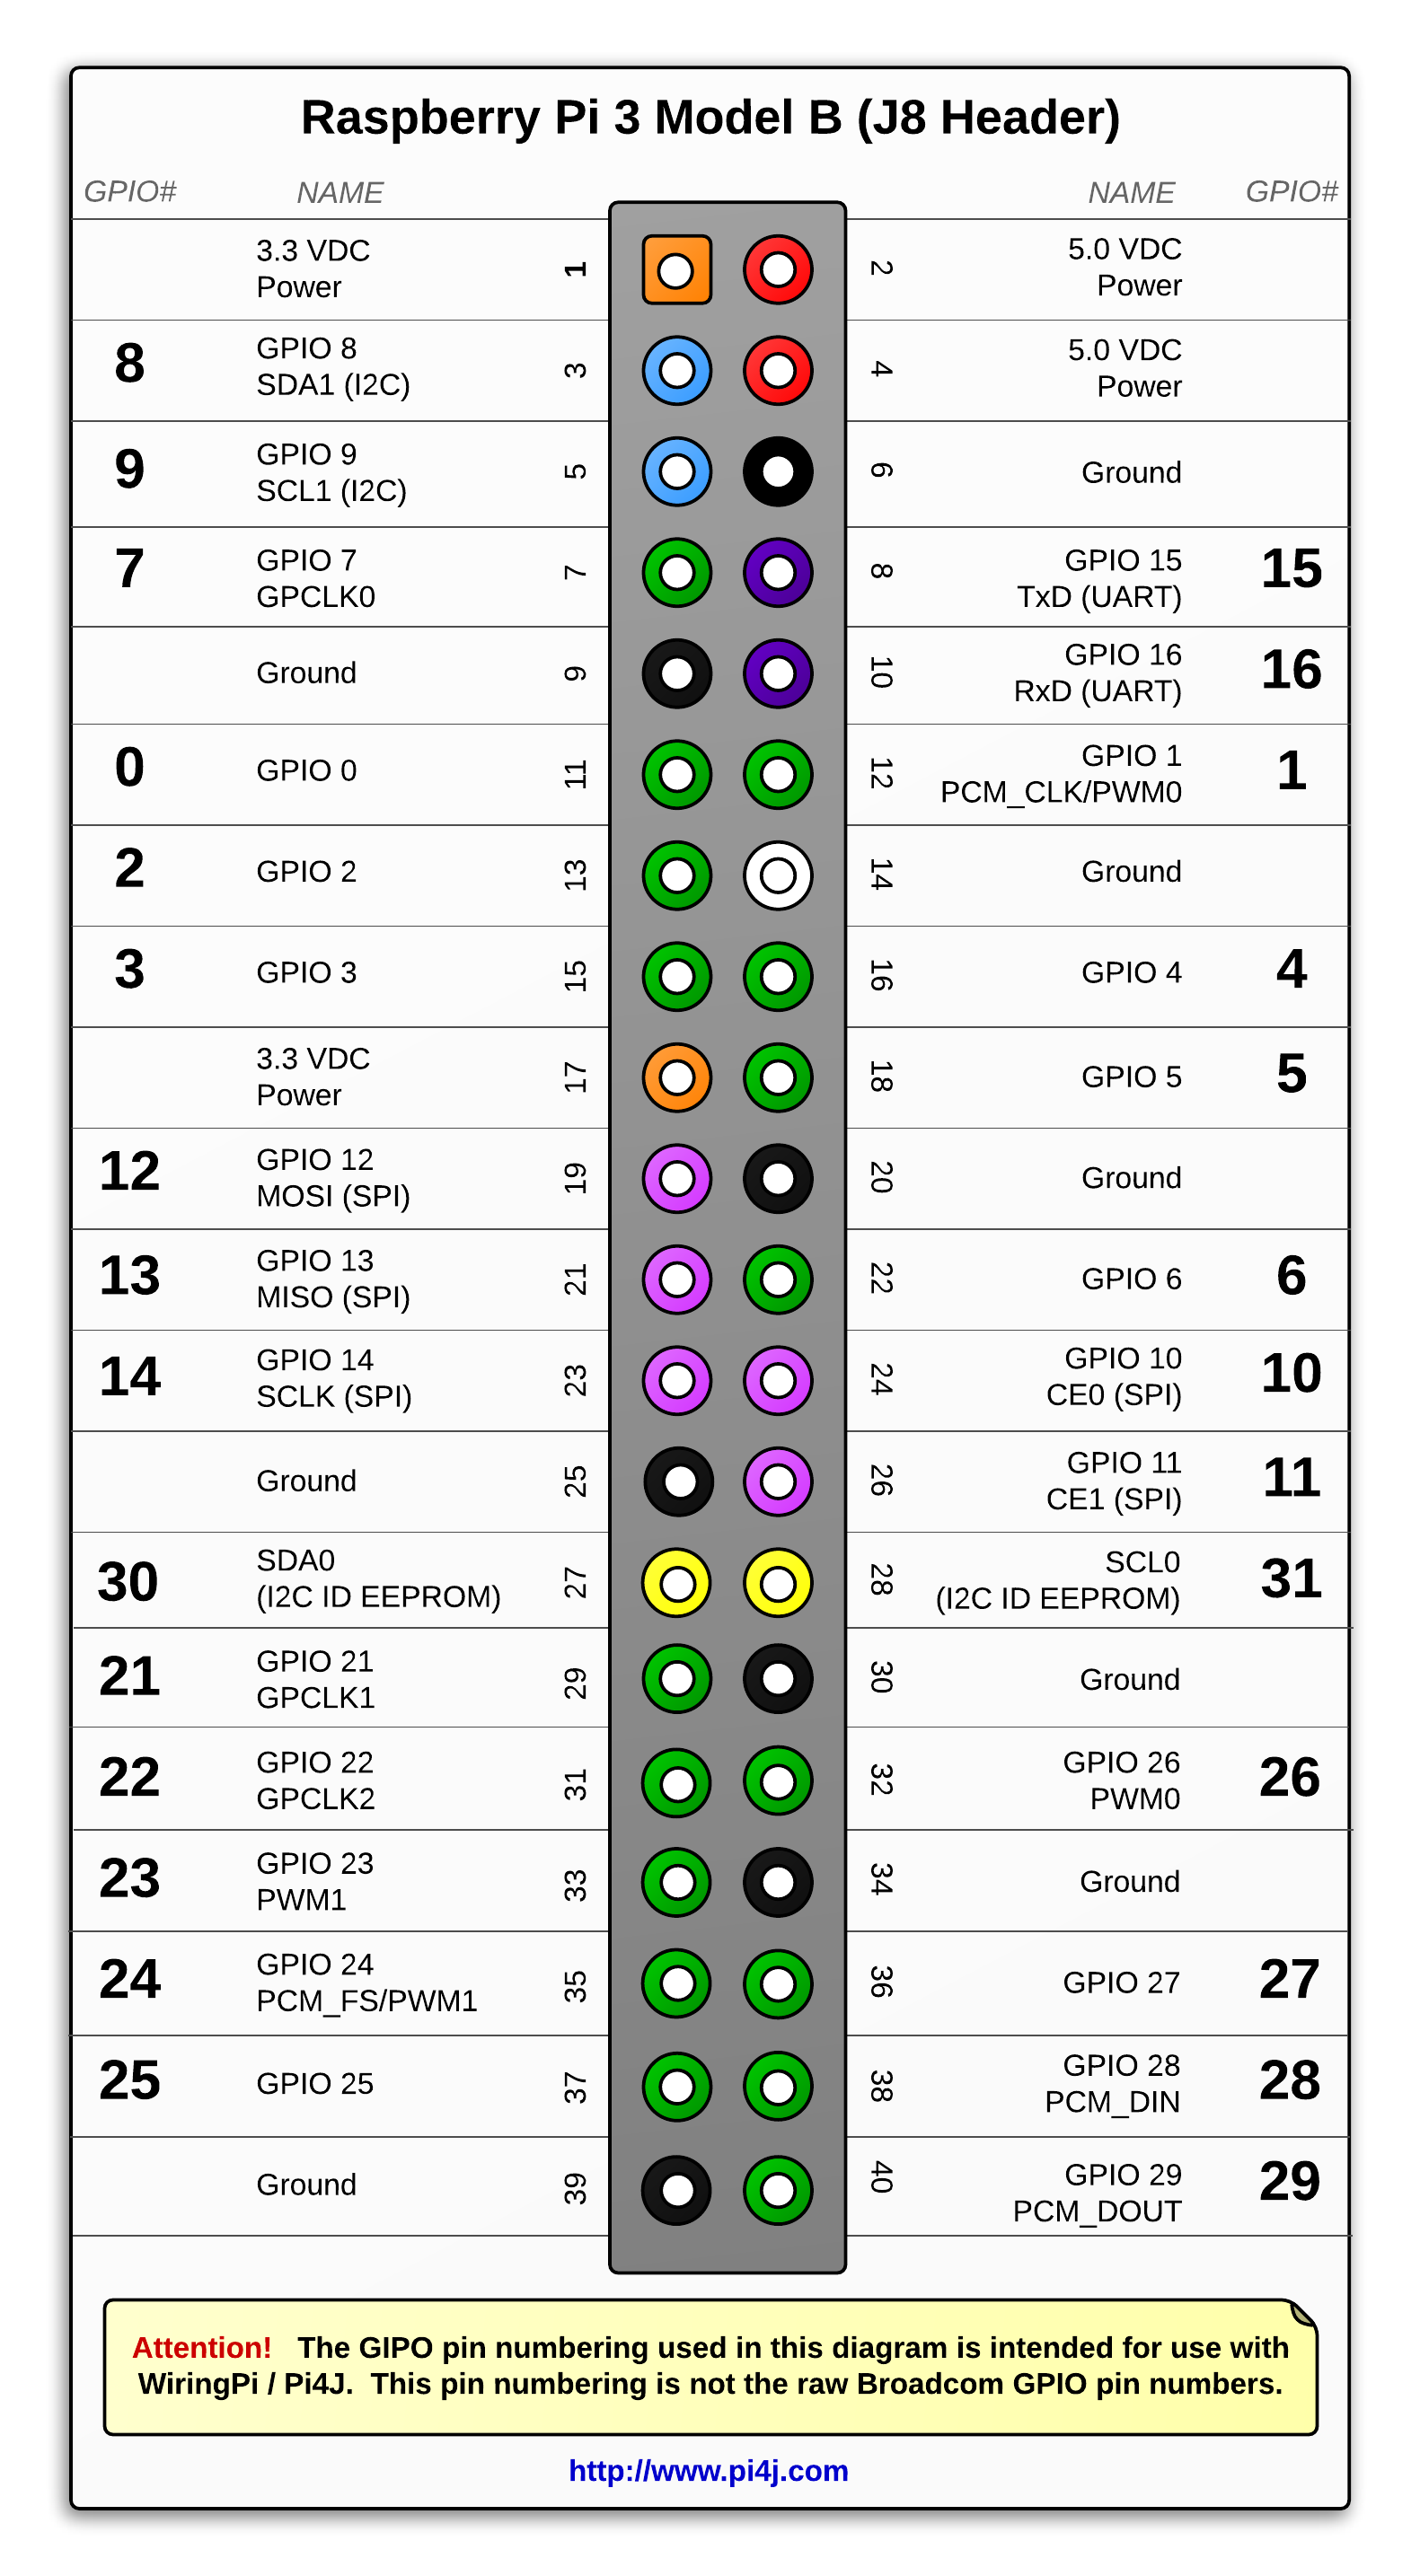
\includegraphics[width=0.42\linewidth]{"./raspberry-pi-3b-pin-diagram-j8header.png"}
				\caption{Raspberry Pi 3B pin diagram}
				\label{fig: Raspberry Pi 3B pin diagram}
			\end{figure}
			
			
			\footnotetext[1]{\label{HardwareSource} Most hardware for this project was obtained from specialty electronic stores around Mumbai. The Raspberry Pi 3B was borrowed from Prof. Bhole, Computers and Information Techonolgy Department, VJTI. We did our best not to alter his existing configurations.}
		
		
		
			
		\clearpage
		
		\item \textbf{Wheels and motors:} 
		
			The robot moves using two wheels each driven by a 300 RPM DC motor. These DC motors are connected with L293D IC which provides and H bridge to turn one motor and other off or both simultaneously in same direction or different direction. 
		
		
		\item \textbf{L293D Motor Driver:} 
		
			A quadruple high-current half-H driver. The L293D is designed to provide bidirectional drive currents of up to 600-mA at voltages from 4.5 V to 36 V. This allows the wheels to move in both directions and also turn left and right. ${}^{\cite{L293D_MotorDriver}}$
		
		
			We connect this driver${}^{\ref{fig: L293D Motor Driver pin diagram}}$ to the following pins of the Raspberry Pi:
	
			\tabulinesep=6pt	% Source: tex.stackexchange.com/a/207146/110560
			\begin{longtabu} to \textwidth {| c | c | } \hline
				\centering 
				Raspberry Pi 3B & L293D \\ \hline
				GPIO 29 (pin 40) & VCC \\ 
				GPIO 28 (pin 38) & GND \\ 
				GPIO 26 (pin 32) & GND \\ 
				Ground (pin 30) & GND \\ \hline
				\caption{Connections of Raspberry Pi to L293D Motor Driver}
			\end{longtabu}
			
			\begin{figure}[!h]
				\centering
				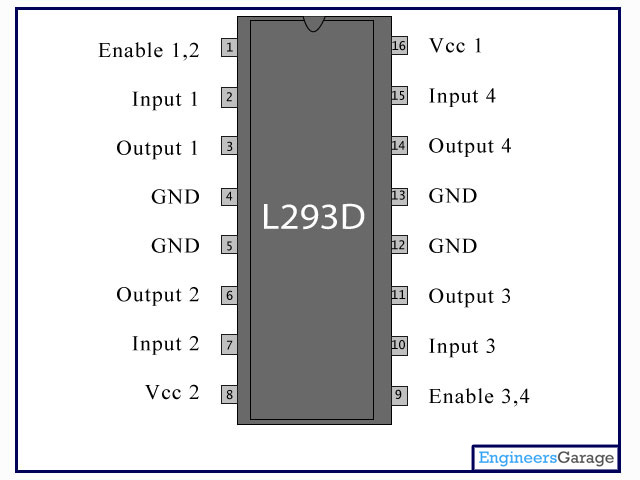
\includegraphics[width=0.5\linewidth]{"./L293D.jpg"}
				\caption{L293D Motor Driver pin diagram}
				\label{fig: L293D Motor Driver pin diagram}
			\end{figure}
			
			
			 \begin{figure}
				\centering
				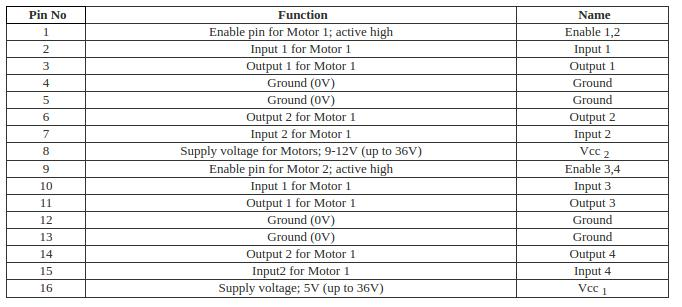
\includegraphics[width=0.9\linewidth]{L293D_pin_description}
				\caption{L293D pin description}
				\label{fig:L293D_pin_description}
			\end{figure}

			 
		 
		\item \textbf{IR sensors:} 
		
			In the rover, IR sensors are used to perform line-following on black or white striped lines. 
		
			IR sensors work on the principle of reflectance where there is one transmitter and one receiver. The transmitter transmits InfraRed rays which are received by the receiver to complete the circuit, due to which current flows through it. ${}^{\ref{fig:IR_transmitter_reciever}}$

			\begin{figure}
				\centering
				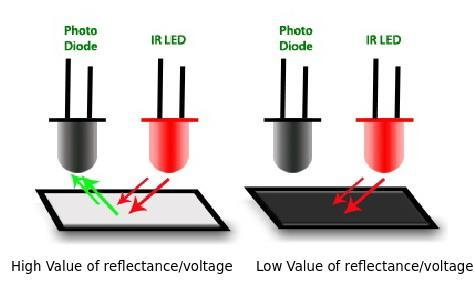
\includegraphics[width=0.6\linewidth]{IR_transmitter_reciever}
				\caption{The working of IR sensors}
				\label{fig:IR_transmitter_reciever}
			\end{figure}
			
			
			Dark colors are good absorber of rays, and they reflect very few of the IR rays falling on it. Due to this phenomenon, using a dark color as the background and white color as line allows to distinguish the path from the background as only white color will be detected by the sensors. 
			
			
			The sensitivity towards black and white of the IR sensor is adjusted by turning the potentiometer knobs on the top of each IR sensor.

	\end{enumerate}
	
	
	
	
	
	
	
	\subsection{Software}
	
	\begin{enumerate}[topsep=-2pt, itemsep=10mm]
		\item \textbf{Raspbian Jesse:} 
		
			It is a full-featured Linux operating system running a version of the Linux kernel and drivers, allowing seamless integration with external hardware such as cameras, ethernet, and Wireless LAN connections. Raspbian is highly optimized for the Raspberry Pi line's low-performance ARM CPUs.
			
			Raspbian uses PIXEL, Pi Improved Xwindows Environment, Lightweight as its main desktop environment as of the latest update. It is composed of a modified LXDE desktop environment and the Openbox stacking window manager with a new theme and few other changes.${}^{\cite{RaspbianPIXEL}}$ 
			
			The Raspbian operating system is based on Debian Linux, and the different versions of Debian are named after characters from the “Toy Story” films.${}^{\cite{RaspbianNaming}}$
		
		
		\item \textbf{Python:} 
		
		
		Python is an open-sourced, general-purpose programming language that is highly suited for writing short scripts without a log of boilerplate. First developed in 1995, it is one of the most popular programming languages that uses \textit{dynamic typing}. Python code files (.py) are compiled down to bytecode to run on the Python \textit{virtual machine}. 
		
		Python is a mainstay in Linux, and it is installed by default in almost all Linux distributions, including Raspbian. Despite it's simplicity, it is very powerful. 
		
		Because of the \textit{RPi} library, integrating Python into robotics experiments using the Raspberry Pi becomes particularly easy. We will often use \textit{RPi.GPIO} to send and receive inputs from the GOPI pins, controlling the motors. 
		
		
		\item \textbf{Django server:}
		
		Django is a high-level Python Web framework that encourages rapid development and clean, pragmatic design. ${}^{\cite{DjangoDescription}}$ It is often used to host large production websites. It is incredibly easy to install, as it is fully encapsulated into a Python library and thus installable with Python \textit{pip} via the command: 
		%Source: http://stackoverflow.com/a/3175170/4900327
		\begin{verbatim}  
			$ pip install django
		\end{verbatim}
		
		It is a testament to the Raspbian OS and the Django project that it is able to run the Django server as an extremely lightweight hosting server, which can be configured to receive requests from other computers on the same Wifi network by binding the runtime to receive requests from a static IP address. 
		
		We use Django to serve the frontend GUI interface on an HTTP GET request, and one clicking a button, we visit the appropriate link (e.g. \url{172.168.42.1/controls/left}) and perform the action specified there. The server imports the \textit{RPi.GPIO} package and sets the pins high or low, depending on the command. This in turn causes the 
		
		We also use the frontend to display the current status of the IR sensors as a string of zeros and ones, such as:
		
		\begin{equation}
			\begin{bmatrix}
			0 & 1 & 1
			\end{bmatrix}
		\end{equation}
		
		Which says the middle and right IR sensors are triggered, meaning that portion of the ground is white or light-colored. We retrieve this information using an AJAX call to \url{172.168.42.1/ir-sensors} and display it on the frontend. We update this value every 0.5 seconds using an AJAX call loop.
		
		
		\item \textbf{Bash:} 
		
		Bash scripts or shell scripts are command-line script files (.sh) which run on the Linux platform, allowing us to perform different OS-level functions using system calls. We specify different arguments and flags to change the behavior of the function called. The executable for these are stored in \url{/usr/bin}
		
		In our rover, we want the server to start automatically on boot, so we must create a shell script which gets the IP address that the raspberry pi is connected to and then runs the Django server from that address, as described in \cite{DjangoSameWifiCode}. This allows computers on the same wifi network as the Pi to connect to the Pi and send requests and receive responses from the Django server, which in turn allows us to control the rover's movement.
		
	\end{enumerate}
	
	